\documentclass{beamer}
\usepackage[utf8]{inputenc}
\usepackage{amsmath}
\usepackage{amsfonts}
\usepackage{amssymb}
\usepackage{graphicx}
\usepackage{polski}
\usepackage{tikz}
\usepackage{calc}
\usepackage{array}

\usetikzlibrary{positioning}
\usetheme{Warsaw}

\title[Biuro~matrymonialne]{System ekspertowy realizujący zadania biura matrymonialnego}
\subtitle{Opis teoretyczny projektu}
\author[Bułka,~Byczyńska,~Czyżniejewski,~Rymuszka]{Aleksandra~Bułka\\Aleksandra~Byczyńska\\Jakub~Czyżniejewski\\Mateusz~Rymuszka}
\institute[MiNI~PW]{Wydział Matematyki i Nauk Informacyjnych\\Politechnika Warszawska}
\date[lato~2019]{\today}

\begin{document}
 
\frame{\titlepage}

\begin{frame}
	\frametitle{Konspekt}
	
	\tableofcontents
	
\end{frame}

\section{Założenia projektowe}

\subsection{Porównanie: kiedyś i dzisiaj}

\begin{frame}

	\begin{block}{Dawniej}
		Pracownik biura matrymonialnego (tutaj: ekspert dziedziny), na podstawie opisu wymagań klienta, odszukiwał osoby, które pasowałyby do preferencji osoby poszukującej partnera
	\end{block}

	\begin{figure}
		\centering
		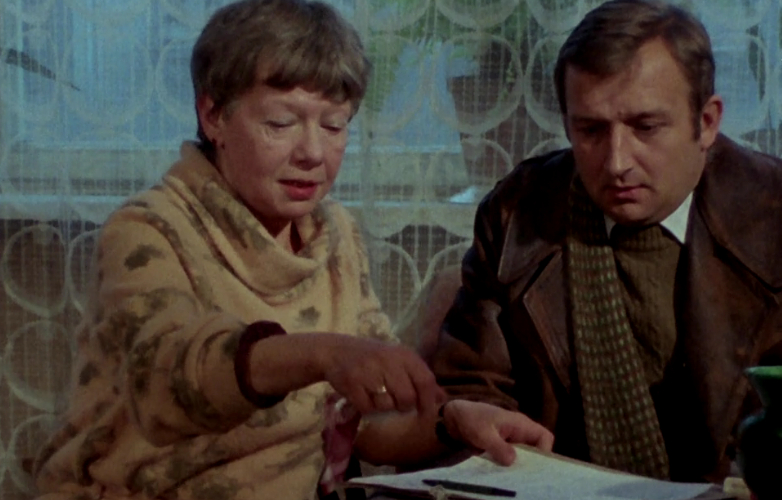
\includegraphics[height=0.5\textheight,keepaspectratio]{images/biuro-kiedys.jpg}
		\caption{Kadr z serialu ``Jan Serce``}
	\end{figure}

\end{frame}

\begin{frame}

	\begin{block}{Dawniej}
		Pracownik biura matrymonialnego (tutaj: ekspert dziedziny), na podstawie opisu wymagań klienta, odszukiwał osoby, które pasowałyby do preferencji osoby poszukującej partnera
	\end{block}
	
	\begin{block}{Wady}
		\begin{itemize}
			\item możliwość zgubienia lub przeoczenia karty klienta
			\item długi czas odszukiwania osób pasujących do rysopisu
			\item subiektywizm osoby wertującej kartotekę
			\item brak powtarzalności procesu
		\end{itemize}
	\end{block}

\end{frame}

\begin{frame}
	
	\begin{block}{Dzisiaj}
		System ekspertowy, po wypełnieniu kwestionariusza przez klienta, automatycznie dopasowuje potencjalnych kandydatów do randkowania
	\end{block}
	
	\begin{figure}
		\centering
		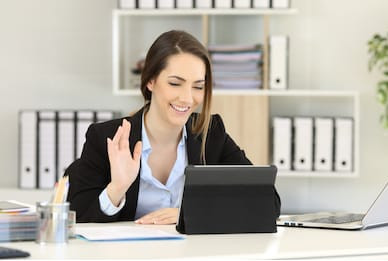
\includegraphics[height=0.5\textheight,keepaspectratio]{images/biuro-dzisiaj.jpg}
		\caption{Biuro matrymonialne obecnie}
	\end{figure}

\end{frame}

\begin{frame}
	
	\begin{block}{Dzisiaj}
		System ekspertowy, po wypełnieniu kwestionariusza przez klienta, automatycznie dopasowuje potencjalnych kandydatów do randkowania
	\end{block}
	
	\begin{block}{Zalety wobec starego systemu}
		\begin{itemize}
			\item wszyscy klienci biura są uwzględnieni 
			\item krótki czas wnioskowania
			\item bezstronność komputera
			\item dyskrecja
		\end{itemize}
	\end{block}

\end{frame}

\subsection{Wymagania biznesowe}

\begin{frame}
	
	\begin{block}{Wymagania biznesowe}
		\begin{itemize}
			\item możliwość natychmiastowego dodawania/edycji/usuwania klientów z bazy biura
			\item wybór najtrafniejszej osoby według preferencji klienta
			\item prezentacja osób spełniający wymagania postawione w formularzu
			\item niezależność logiki wnioskowania od bazy wiedzy
			\item jasny i przejrzysty interfejs użytkownika
		\end{itemize}
	\end{block}

\end{frame}

\section{Opis architektury systemu}

\subsection{Schemat architektury}

\begin{frame}
	\begin{figure}
		\centering
		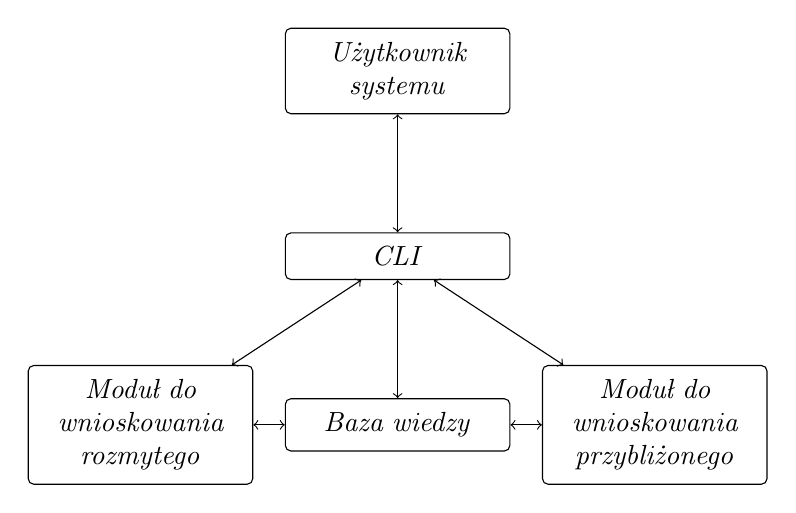
\begin{tikzpicture}[
				rounded corners=2pt,
				inner sep=5pt,
				node distance=1.5cm,
				text width=2.5cm,
				align=center
			]
			
			\node [draw] (user) {\textit{Użytkownik systemu}};
			\node [draw,below=of user] (cli) {\textit{CLI}};
			\node [draw,below=of cli] (database) {\textit{Baza wiedzy}};
			\node [draw,left=.4cm of database] (fuzzy) {\textit{Moduł do wnioskowania rozmytego}};
			\node [draw,right=.4cm of database] (rough) {\textit{Moduł do wnioskowania przybliżonego}};
			
			\draw [<->] (user) -- (cli);
			\draw [<->] (cli) -- (fuzzy);
			\draw [<->] (cli) -- (database);
			\draw [<->] (cli) -- (rough);
			\draw [<->] (database) -- (fuzzy);
			\draw [<->] (database) -- (rough);
		\end{tikzpicture}
		\caption{\centering Schemat architektury systemu eksperckiego biura matrymonialnego}
	\end{figure}
	
\end{frame}

\subsection{Opis modułów systemowych}

\begin{frame}

	\begin{block}{Moduły wnioskowania}
		Moduły wnioskowania będą zawierać klauzule definiujące fakty i reguły odpowiadające za wnioskowanie na podstawie bazy wiedzy. 
		
		Zespół zaimplementuje:
		\begin{itemize}
			\item moduł wnioskowania przybliżonego - wyznaczający reguły decyzyjne w oparciu o teorię zbiorów przybliżonych
			\item moduł wnioskowania rozmytego - wyznaczający reguły decyzyjne w oparciu o logikę rozmytą
		\end{itemize}
	\end{block}

\end{frame}

\begin{frame}

	\begin{block}{Baza wiedzy}
		Osobny moduł będzie stanowiła baza wiedzy. Można podzielić ją na:
		\begin{itemize}
			\item część statyczną, z podstawowymi faktami i regułami na temat systemu
			\item część dynamiczną, ładowaną z pliku lub modyfikowaną przez obsługującego
		\end{itemize}
		Zespół przygotuje zarówno predykaty statycznej bazy wiedzy oraz interfejs do zarządzania dynamiczną bazą danych.
	\end{block}

\end{frame}

\begin{frame}
	
	\begin{block}{Interfejs użytkownika}
		Do aplikacji zostanie przygotowany prosty interfejs użytkownika. Będzie spoiwem łączącym wszystkie funkcjonalności systemu, tzn. będzie umożliwiał zarówno delegację zadań do modułu zarządzania bazą wiedzy oraz rozpoczęcie procesu wnioskowania na podstawie faktów podanych przez użytkownika. 
		
		Interfejs będzie umożliwiał komunikację za pomocą konsoli (tzw. CLI - \textit{ang. Command Line Interface}).
	\end{block}

\end{frame}

\section{Wnioskowanie}

\subsection{Metody wnioskowania}

\begin{frame}

\end{frame}

\subsection{Przykłady reguł w systemie}

\begin{frame}

\end{frame}

\subsection{Przykład działania programu}

\begin{frame}

\end{frame} 

\end{document}


